\rchapter{Acceleration with Pyccel}

\section{Introduction}

As mentioned in chapter \ref{chapter::Introduction} python runs much slower than compiled languages. Tests on the code produced thus far at first did not yield results. Once the total size of the simulation was reduced by a factor of eight, it was found that five time steps could be run on one node containing 32 processes in three hours. This means that the full simulation would take more than a year and a half to run on one node. Assuming perfect scaling, it would take nearly 5 days on the theoretical maximum number of processes (4096 processes, 128 nodes), and nearly 20 days on the maximum number of processes allowed by the supercomputer used (1024 processes, 32 nodes). These times are unreasonable, especially if the simulation must be rerun. It is therefore important to find a way to accelerate the code.

Pyccel \cite{Pyccel} is one tool that can be used to accelerate python code. It translates the python code into human readable Fortran code. This code can then be compiled and f2py can be used to allow the accelerated version to be called from python. This allows bottlenecks to be run at faster speeds without the code needing to be written in Fortran. It also means that the majority of the code is still written in python which can make it easier to understand. In addition the readability of the Fortran code allows the generated files to be easily modified to exploit any advantages of Fortran which cannot be mimicked in python.

\section{Using Pyccel}

A function can be pyccelised if it contains only basic python and numpy methods\footnote{Not all methods are currently supported by pyccel}. As classes cannot be pyccelised, functions must be created containing the pyccelisable content. These can then be called from the class to mask the larger interface that this creates.

Once the functions to be pyccelised have been selected, the pyccelisation can begin. All functions which will be called directly should be placed in one file. All functions which are used by those functions are then placed in a second file whose name must have the form ``mod\_[XX].py'', where [XX] can be anything. The ``mod\_[XX].py'' is used by epyccel, the interactive version of pyccel, as a context, enabling it to generate a shared object file. All functions must also be given a header specifying the Fortran types of the arguments. The header can either take the form of a comment or a function decorator. Function decorators are preferable as they can be imported interactively with the function. The syntax is as follows:

\begin{lstlisting}[language=python,style=pythonStyle]
 #$ header function my_function(double,int,double[:],int[:,:])
 @types('double','int','double[:]','int[:,:]')
\end{lstlisting}

Once the functions have been assembled in the correct files and given the appropriate headers, the context must be compiled. To do this one can use the command:

\begin{lstlisting}[language=bash,style=bashStyle]
 pyccel mod_[XX].py --fflags ' -O3 -fPIC'
\end{lstlisting}

The Fortran flags must be specified to ensure that the resulting files can be converted with f2py. If one wishes to generate the pyccel file from a different folder, then this can be done with the following command

\begin{lstlisting}[language=bash,style=bashStyle]
 pyccel folder1/folder2/mod_[XX].py --output folder1/folder2   --fflags ' -O3 -fPIC'
\end{lstlisting}

This allows all files to be generated simply from one location. This is the version which is used in this project.

Alternatively if the generated Fortran code may be modified then the chosen pyccel command should be given the flag '-t'. The generated code must then be compiled. For example the following command must be used with the gfortran or intel compiler respectively:

\begin{lstlisting}[language=bash,style=bashStyle]
 gfortran -O3 -fPIC -c folder1/folder2/mod_[XX].f90 -o folder1/folder2/mod_[XX].o  -J folder1/folder2/
 ifort -O3 -fPIC -c folder1/folder2/mod_[XX].f90 -o folder1/folder2/mod_[XX].o  -module folder1/folder2/
\end{lstlisting}

Once the context file is prepared then a shared object file can be generated using epyccel. In order to do this the module to be pyccelised and the functions from the context file must be imported. A ContextPyccel object should then be created containing all the functions required, and the types of their arguments. If the pyccelisation is carried out from a folder which does not contain the modules then the position of the module in the python hierarchy must be specified using the context\_folder keyword. The following code, showing the commands required to generate the shared object for the spline module, serves as an example:

\begin{lstlisting}[language=python,style=pythonStyle]
from pyccel.epyccel import ContextPyccel
from pyccel.epyccel import epyccel

import pygyro.splines.spline_eval_funcs
from pygyro.splines.mod_context_1 import find_span,basis_funs,basis_funs_1st_der

spline_context = ContextPyccel(name='context_1', context_folder='pygyro.splines')
spline_context.insert_function(find_span, ['double[:]','int','double'])
spline_context.insert_function(basis_funs, ['double[:]','int','double','int','double[:]'])
spline_context.insert_function(basis_funs_1st_der, ['double[:]','int','double','int','double[:]'])

spline_eval_funcs = epyccel(pygyro.splines.spline_eval_funcs, context=spline_context)
\end{lstlisting}


\section{Spline Acceleration}

In order to reap maximum benefits from the acceleration it is important to accelerate the functions which take the most time. These act as a bottleneck for the program. In order to determine which functions these are, the python profiler cProfile will be used on a personal laptop to examine the performance of the program using a grid with 10 grid points in each dimension. Three processes are used and the results are averaged over each process. The results for the pure python implementation are shown in table \ref{tab::pure python profile}.

\begin{table}[ht]
 \begin{tabular}{|m{.37\textwidth}|c|c|c|c|}
  \hline
          & Total time & Number & Time & Total \\
  Function & excluding sub & of & per call & time \\
          & functions [s] & calls & [s] & [s] \\
  \hline
  \hline
  method 'Alltoall' from mpi4py & 28.193 & 250 & 0.113 & 28.193 \\
  \hline
  numpy.core.multiarray.array & 16.070 & 5689347 & 0.000 & 16.070 \\
  \hline
  bisplev from scipy & 10.009 & 1006666 & 0.000 & 37.819\\
  \hline
  method scipy.interpolate. \_fitpack.\_bispev & 8.503 & 1006666 & 0.000 & 8.503\\
  \hline
  atleast\_1d from numpy & 7.990 & 2915166 & 0.000 & 23.820\\
  \hline
  splev & 7.334 & 901833 & 0.000 & 18.883\\
  \hline
  reshape from numpy & 6.590 & 3397927 & 0.000 & 6.590\\
  \hline
 \end{tabular}
\caption{\label{tab::pure python profile} The results of profiling the pure python implementation}
\end{table}

We note firstly that the slowest function is mpi4py’s Alltoall function. This is due to the small size of the grid which means that calculations can run faster, and the fact that the tests were run on 3 processes. This leads to a poor data balance as 2 processes have 3x10x10x10 sized grids and the third has a 4x10x10x10 sized grid. As a collective operation Alltoall therefore is obliged to wait until all processes have reached the same point. These problems will not apply when the full simulation is run so this function will not be accelerated. 

The second bottleneck is due to internal numpy functions. There is nothing that can be done about this directly although it can be hoped that accelerating other functions will lead to less reliance on numpy which will therefore eliminate this bottleneck.

The next four bottlenecks all arise due to the implementation of the splines. Bisplev is a scipy function which calls bispev in order to evaluate a 2d spline while splev is its 1d equivalent. The reshape command is used to flatten the 2D array containing the coefficients for the bisplev function, as well as during all layout changes. The function atleast\_1d  is  only used explicitly during the initialisation, which is not profiled. This means that the function must be called implicitly,  probably by one of the scipy functions. The eval functions of the classes Spline1D and Spline2D are therefore the functions which will be accelerated first.

In order to accelerate these two functions a mod\_context\_1.py file will be created. This file will contain the functions find\_span, basis\_funs, and basis\_funs\_1st\_der. These functions are obtained from the SPL library \cite{python_spl}.  In addition a spline\_eval\_funcs.py file will be created. The file will contain the functions eval\_spline\_1d\_scalar, eval\_spline\_1d\_vector, eval\_spline\_2d\_scalar, and eval\_spline\_2d\_cross which mimic the behaviour of the scipy functions splev and bisplev. Furthermore a function eval\_spline\_2d\_vector will be added to help avoid unaccelerated Python loops. The scipy function calls will then be replaced by an if statement which verifies whether the input has a length, and a call to the necessary function. This implementation ensures that calls elsewhere in the program do not need to be modified. It may however slow the program somewhat as it adds additional function calls which are unnecessary if the type of the data is known.

The results of the acceleration can be seen in table \ref{tab::spline profile}. It can be seen that although the spline calls remain some of the most costly function calls, the total time spent in each function is significantly reduced. For example in the case of the 2D spline evaluation, previously 37.8 seconds were spent in the function bisplev and its sub-functions, in contrast now only 12.3 seconds are spent in eval in total. Similarly the 1D spline evaluation previously required 18.8 seconds and now takes only 6.3 seconds.

\begin{table}[ht]
\centering
 \begin{tabular}{|m{.37\textwidth}|c|c|c|c|}
  \hline
          & Total time & Number & Time & Total \\
  Function & excluding sub & of & per call & time \\
          & functions [s] & calls & [s] & [s] \\
  \hline
  \hline
  method 'Alltoall' from mpi4py & 10.461 & 250 & 0.042 & 10.461 \\
  \hline
  numpy.core.multiarray.array & 9.340 & 1624947 & 0.000 & 9.340 \\
  \hline
  eval in Spline2D & 7.225 & 1006666 & 0.000 & 12.345\\
  \hline
  step in PoloidalAdvection & 5.423 & 3333 & 0.002 & 35.266\\
  \hline
  eval in Spline1D & 4.948 & 901833 & 0.000 & 6.319\\
  \hline
  step in FluxSurfaceAdvection & 4.744 & 5000 & 0.001 & 9.527\\
  \hline
  \_vectorize\_call & 4.403 & 383333 & 0.000 & 25.365\\
  \hline
 \end{tabular}
 \caption{\label{tab::spline profile} The results of profiling the implementation after the acceleration of the spline functions}
\end{table}

\section{Initialisation Acceleration}

The profiling results will once more be used to determine which functions should be accelerated. The slowest functions are the eval functions of the Spline1D and Spline2D classes, the poloidal advection and the flux surface advection. These functions call the eval functions. As part of the acceleration they can call the previously accelerated functions directly.

The advection steps use the expression for the equilibrium distribution at the boundaries. As a result, the initialisation functions must first be accelerated in order to accelerate the advection equations.

Unfortunately, unlike the splines, the initialisation cannot be accelerated while keeping the old file access patterns. The initialisation takes advantage of the flexibility of numpy which can handle both scalar and vector functions however Fortran does not have this flexibility. In order to avoid loosing speed the files will therefore be organised such that a file called mod\_initialiser\_funcs.py will be created containing all scalar functions and a file called initialiser\_func.py will be created to handle the vector case by looping over the scalar function. mod\_initialiser\_funcs.py will also be used as a context for the advection.

\begin{table}[ht]
\centering
 \begin{tabular}{|m{.37\textwidth}|c|c|c|c|}
  \hline
          & Total time & Number & Time & Total \\
  Function & excluding sub & of & per call & time \\
          & functions [s] & calls & [s] & [s] \\
  \hline
  \hline
  method 'Alltoall' from mpi4py & 20.373 &  250 & 0.081 & 20.373 \\
  \hline
  numpy.core.multiarray.array & 9.581 &   1872347 & 0.000 & 9.581 \\
  \hline
  eval in Spline2D & 7.423 &   1006666 & 0.000 & 12.722\\
  \hline
  step in PoloidalAdvection & 5.639 &      3333 & 0.002 & 42.126\\
  \hline
  eval in Spline1D & 5.211 & 910400 & 0.000 & 6.655\\
  \hline
  step in FluxSurfaceAdvection & 4.802 & 5000 & 0.001 & 9.772\\
  \hline
  \_vectorize\_call & 4.538 & 383333 & 0.000 & 25.898\\
  \hline
 \end{tabular}
 \caption{\label{tab::init profile} The results of profiling the implementation after the acceleration of the spline and initialisation functions}
\end{table}

As the accelerated functions are used in the initialisation which is not profiled we do not expect to see a change in the results after these improvements. The new results of profiling are shown in table \ref{tab::init profile} and are as expected.

\section{Advection Acceleration}

\begin{table}[ht]
\centering
 \begin{tabular}{|m{.37\textwidth}|c|c|c|c|}
  \hline
          & Total time & Number & Time & Total \\
  Function & excluding sub & of & per call & time \\
          & functions [s] & calls & [s] & [s] \\
  \hline
  \hline
  method 'Alltoall' from mpi4py & 4.361 & 250 & 0.017 & 4.361 \\
  \hline
  step in FluxSurfaceAdvection & 1.874 & 5000 & 0.000 & 3.428 \\
  \hline
  step in PoloidalAdvection & 1.489 & 3333 & 0.000 & 3.135\\
  \hline
  method 'solve' from scipy 'SuperLU' object & 1.330 & 96666 & 0.000 & 1.330\\
  \hline
  getPerturbedRho in ParallelGradient & 1.221 & 101 & 0.012 & 5.407\\
  \hline
  parallel\_gradient in ParallelGradient & 1.213 & 1000 & 0.001 & 2.348\\
  \hline
  \_solve\_system\_nonperiodic in SplineInterpolator1D & 1.109 & 123700 & 0.000 & 1.109\\
  \hline
 \end{tabular}
 \caption{\label{tab::adv profile} The results of profiling the implementation after the acceleration of the spline, initialisation, and advection functions}
\end{table}

We are now able to accelerate the advection functions. We begin by accelerating the poloidal advection. The files written for the splines and the initialisation are used to provide a context for the accelerated advection file. Unfortunately a context cannot have its own context. Thus a file mod\_spline\_eval\_funcs.py must be created containing the contents of mod\_context\_1.py and spline\_eval\_funcs.py.

Once this step has been accomplished successfully the pyccelisable parts of the v-parallel and flux surface advections can be added to the accelerated advection file very simply.

The results of the profiling after this pyccelisation can be seen in table \ref{tab::adv profile}. Although the advection steps are still the slowest steps we note that while previously 42.1 seconds were spent in the PoloidalAdvection step and its sub-function, now only 3.1 seconds are required. Similarly while previously 9.8 seconds were spent in the FluxSurfaceAdvection step and its sub-functions, now only 3.4 seconds are required.

The remaining functions are harder to accelerate. They each contain very little code, but call 'eval' from Spline1D multiple times. This allows for a small improvement as it is possible to call the accelerated function directly without using Spline1D. This avoids the type check which decides whether to use the scalar or vector version of the accelerated function. An additional improvement was found in 'getPerturbedRho' by calculating the value of the distribution function at equilibrium in the initialisation, thus avoiding recalculating it at each step.

\begin{table}[ht]
\centering
 \begin{tabular}{|m{.37\textwidth}|c|c|c|c|}
  \hline
          & Total time & Number & Time & Total \\
  Function & excluding sub & of & per call & time \\
          & functions [s] & calls & [s] & [s] \\
  \hline
  \hline
  method 'Alltoall' from mpi4py & 2.735 & 250 & 0.011 & 2.735 \\
  \hline
  step in FluxSurfaceAdvection & 1.826 & 5000 & 0.000 & 3.355 \\
  \hline
  parallel\_gradient in ParallelGradient & 1.492 & 1000 & 0.001 & 1.903\\
  \hline
  step in PoloidalAdvection object & 1.420 & 3333 & 0.000 & 3.004\\
  \hline
  method 'solve' from scipy 'SuperLU' & 1.294 & 96666 & 0.000 & 1.294\\
  \hline
  getPerturbedRho in ParallelGradient & 1.022 & 101 & 0.010 & 2.307\\
  \hline
  \_solve\_system\_nonperiodic in SplineInterpolator1D & 0.977 & 123700 & 0.000 & 0.977\\
  \hline
 \end{tabular}
 \caption{\label{tab::final profile} The results of profiling the implementation after the acceleration of the spline, initialisation, and advection functions}
\end{table}

The profile after these final improvements can be seen in table \ref{tab::final profile}. Note that the improvements have slowed the parallel\_gradient function as the calls are more complicated but the overall time spent in this function and its sub-functions is still greatly reduced. Note also that the bottleneck due to the numpy internal functions has also disappeared as hoped.

\section{Results}

Having accelerated the functions on a personal laptop, it is important to verify that the results hold for the full grid on the supercomputer. Table \ref{tab::draco profile} show the averaged results of profiling the full 256x512x32x128 grid on one node with 32 processes. The results are very similar to those seen in table \ref{tab::adv profile}. This shows that this method was sufficient for finding the bottlenecks.

\begin{table}[ht]
\centering
 \begin{tabular}{|m{.37\textwidth}|c|c|c|c|}
  \hline
          & Total time & Number & Time & Total \\
  Function & excluding sub & of & per call & time \\
          & functions [s] & calls & [s] & [s] \\
  \hline
  \hline
  step in FluxSurfaceAdvection & 522.026 & 15360 & 0.034 & 579.579 \\
  \hline
  step in PoloidalAdvection & 510.948 & 1280 & 0.399 & 559.224 \\
  \hline
  getPerturbedRho in ParallelGradient & 184.991 & 11 & 16.817 & 231.574 \\
  \hline
  method 'Alltoall' from mpi4py & 108.146 & 78 & 1.386 & 108.146 \\
  \hline
  step in VParallelAdvection & 102.033 & 1966080 & 0.000 & 131.171 \\
  \hline
  method 'solve' from scipy 'SuperLU' object & 82.426 & 849920 & 0.000 & 82.426 \\
  \hline
  \_solve\_system\_nonperiodic in SplineInterpolator1D & 50.279 & 4109824 & 0.000 & 50.279 \\
  \hline
 \end{tabular}
 \caption{\label{tab::draco profile} The results of profiling the implementation on one node of the supercomputer after accelerating the functions}
\end{table}

Note that the mpi 'Alltoall' command no longer dominates the simulation. This is due to better balancing and a better calculation to communication ratio. Instead the advection steps are by far the biggest bottleneck. If any further improvements are required, they would therefore ideally be found in these functions.

The performance of the generated code depends on the compiler used. For the profiling, gfortran was always used, however on the supercomputer the results can also be tested using the intel compiler. The improvements obtained are shown in table \ref{tab::timings}.

The pure Fortran implementation referenced is that used by Latu et al.\cite{YamanPaper} for their work on the same problem. Although the best pyccel version is still three times slower than the pure Fortran version, it still runs at an acceptable speed. The speed of development also makes this increase easily justifiable. In addition there is still scope for improvement. The generated code could be improved, for example by indicating which functions are 'pure', or by using more compiler flags. The algorithms could also be modified to increase the speed. For example the implementation of the spline evaluation is very general however the points are equidistant in all cases, except for points close to the boundary along an axis which does not have periodic boundary conditions. This knowledge can be exploited to produce faster code, as is done in the pure Fortran version.

\begin{table}[H]
\centering
 \begin{tabular}{|c|c|c|}
  \hline
  Version & Time per step [s] & Improvement\\
  \hline
  Pure Python & 17748\footnotemark & - \\
  \hline
  Pyccel accelerated & 487.6 & 36.4 \\
  (intel) & & \\
  \hline
  Pyccel accelerated & 342.5 & 51.8\\
  (gfortran) & & \\
  \hline
  Modified pyccel & 153.2\footnotemark & 115.8 \\
  accelerated (gfortran) & & \\
  \hline
  Pure Fortran & 122.7 & 144.7\\
  \hline
 \end{tabular}
\caption{\label{tab::timings} Time required to carry out one calculation step on one node containing 32 processes for various versions of the simulation, and the improvement that this represents compared to the pure python version}
\end{table}
\footnotetext[2]{Approximated from the timings using a smaller grid and only 5 timesteps}
\footnotetext{Approximated from the timings using only 5 timesteps}

In addition the parallelisation method allows more processes to be used in the python version than in the original Fortran version. While the Fortran version is limited to 256 processes, the python version can use up to 4096 processes. Figure \ref{fig::Timing Comparison} shows the timings for the various versions and shows that this advantage means that the pyccel accelerated code, accelerated using gfortran can run faster than the Fortran code if it uses 1024 processes. Unfortunately results cannot be shown on more processes as the available supercomputers either did not have the required packages or did not allow programs running on more than 32 nodes.

\begin{figure}[ht]
 \centering
 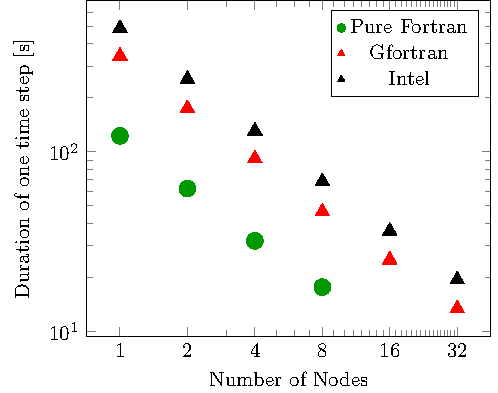
\includegraphics[width=.7\textwidth]{Figs/PythonScaling/Speeds}
 \caption{\label{fig::Timing Comparison}Comparison of time required to carry out one calculation step on different numbers of nodes, each containing 32 processes }
\end{figure}

A first attempt was made to manually improve the code generated by pyccel by avoiding unnecessary calls to the allocate routine and by marking functions as pure. Unfortunately due to time restrictions the results of this improvement cannot be fully presented. However figure \ref{fig::Timing Comparison} and table \ref{tab::timings} are still able to present a first estimation of the effect that these improvements would have. We see that the resulting code is now only 1.2 times slower than the pure Fortran code. This is an excellent result which clearly demonstrates that this development method is a good alternative to developing in Fortran. In addition the changes made were relatively simple, it is therefore hoped that a more mature version of pyccel would be able to generate code with these changes already made.

The new code was also profiled on a personal laptop, and the results can be seen in table \ref{tab::yaman profile}. We note that the bottleneck is now the parallel\_gradient function which has so far received little attention. This may imply that there is scope for further improvements.

\begin{table}[ht]
\centering
 \begin{tabular}{|m{.37\textwidth}|c|c|c|c|}
  \hline
          & Total time & Number & Time & Total \\
  Function & excluding sub & of & per call & time \\
          & functions [s] & calls & [s] & [s] \\
  \hline
  \hline
  method 'Alltoall' from mpi4py & 2.424 & 250 & 0.010 & 2.424 \\
  \hline
  parallel\_gradient in ParallelGradient & 1.450 & 1000 & 0.001 & 1.879 \\
  \hline
  method 'solve' from scipy 'SuperLU' & 1.317 & 96666 & 0.000 & 1.317 \\
  \hline
  step in FluxSurfaceAdvection & 1.101 & 5000 & 0.000 & 2.667 \\
  \hline
  \_solve\_system\_nonperiodic in SplineInterpolator1D & 1.041 & 123700 & 0.000 & 1.041 \\
  \hline
  compute\_interpolant in SplineInterpolator1D & 0.993 & 220366 & 0.000 & 4.285\\
  \hline
  step in VParallelAdvection & 0.938 & 50000 & 0.000 & 1.732\\
  \hline
 \end{tabular}
 \caption{\label{tab::yaman profile} The results of profiling the implementation after manually improving the code generated by pyccel}
\end{table}